\shortdescription{In this activity we practice evaluating functions at numbers and other functions.} % A one sentence description of the activity
\activitytitle{Evaluating Functions} % the title of the activity
\prerequisites{algebra}
\outcomes{functions}


We'll start off easy, asking you a set of questions that you can
probably do.

%%%%%%%%%%%%%%%%%%%%%%%%%%%%%%%%%%%%%%%%%%%%%%%%%%%%%%%%%%%%
%%%%%%%%%%%%%%%%%%%%%%%%%%%%%%%%%%%%%%%%%%%%%%%%%%%%%%%%%%%%
%% Problem
%%%%%%%%%%%%%%%%%%%%%%%%%%%%%%%%%%%%%%%%%%%%%%%%%%%%%%%%%%%%
%%%%%%%%%%%%%%%%%%%%%%%%%%%%%%%%%%%%%%%%%%%%%%%%%%%%%%%%%%%%

\begin{shuffle}
\begin{exercise}
Given that $s(k)=-k^2-4 k+2$, evaluate $s(4.5)$. Express your answer in decimal notation.
\begin{solution}
\begin{hint}
$s(4.5)=-(4.5)^2-4 (4.5)+2$.
\end{hint}
\begin{hint}
$s(4.5)=-36.25$.
\end{hint}
The value of the function $s(k)=-k^2-4 k+2$, evaluated at $k=4.5$, is $\answer{-36.25}$.
\end{solution}
\end{exercise}

\begin{exercise}
Given that $p(u)=2 u^2+3 u-3$, evaluate $p(1.3)$. Express your answer in decimal notation.
\begin{solution}
\begin{hint}
$p(1.3)=2 (1.3)^2+3 (1.3)-3$.
\end{hint}
\begin{hint}
$p(1.3)=4.28$.
\end{hint}
The value of the function $p(u)=2 u^2+3 u-3$, evaluated at $u=1.3$, is $\answer{4.28}$.
\end{solution}
\end{exercise}

\begin{exercise}
Given that $y(u)=u^4+3 u^2-5$, evaluate $y(-3.8)$. Express your answer in decimal notation.
\begin{solution}
\begin{hint}
$y(-3.8)=(-3.8)^4+3 (-3.8)^2-5$.
\end{hint}
\begin{hint}
$y(-3.8)=246.834$.
\end{hint}
The value of the function $y(u)=u^4+3 u^2-5$, evaluated at $u=-3.8$, is $\answer{246.834}$.
\end{solution}
\end{exercise}

\begin{exercise}
Given that $P(z)=2 z^3-3 z^2-3$, evaluate $P(-0.4)$. Express your answer in decimal notation.
\begin{solution}
\begin{hint}
$P(-0.4)=2 (-0.4)^3-3 (-0.4)^2-3$.
\end{hint}
\begin{hint}
$P(-0.4)=-3.608$.
\end{hint}
The value of the function $P(z)=2 z^3-3 z^2-3$, evaluated at $z=-0.4$, is $\answer{-3.608}$.
\end{solution}
\end{exercise}

\begin{exercise}
Given that $F(n)=n^4+n^2-4 n-4$, evaluate $F(-2)$. Express your answer in decimal notation.
\begin{solution}
\begin{hint}
$F(-2)=(-2)^4+(-2)^2-4 (-2)-4$.
\end{hint}
\begin{hint}
$F(-2)=24$.
\end{hint}
The value of the function $F(n)=n^4+n^2-4 n-4$, evaluated at $n=-2$, is $\answer{24}$.
\end{solution}
\end{exercise}

\begin{exercise}
Given that $a(t)=-t-5$, evaluate $a(4.5)$. Express your answer in decimal notation.
\begin{solution}
\begin{hint}
$a(4.5)=-(4.5)-5$.
\end{hint}
\begin{hint}
$a(4.5)=-9.5$.
\end{hint}
The value of the function $a(t)=-t-5$, evaluated at $t=4.5$, is $\answer{-9.5}$.
\end{solution}
\end{exercise}

\begin{exercise}
Given that $Y(v)=-v^4+4 v+4$, evaluate $Y(3.5)$. Express your answer in decimal notation.
\begin{solution}
\begin{hint}
$Y(3.5)=-(3.5)^4+4 (3.5)+4$.
\end{hint}
\begin{hint}
$Y(3.5)=-132.063$.
\end{hint}
The value of the function $Y(v)=-v^4+4 v+4$, evaluated at $v=3.5$, is $\answer{-132.063}$.
\end{solution}
\end{exercise}

\begin{exercise}
Given that $f(n)=-n^2-2 n-2$, evaluate $f(4.7)$. Express your answer in decimal notation.
\begin{solution}
\begin{hint}
$f(4.7)=-(4.7)^2-2 (4.7)-2$.
\end{hint}
\begin{hint}
$f(4.7)=-33.49$.
\end{hint}
The value of the function $f(n)=-n^2-2 n-2$, evaluated at $n=4.7$, is $\answer{-33.49}$.
\end{solution}
\end{exercise}

\begin{exercise}
Given that $B(x)=-x^4+x^3-x^2-1$, evaluate $B(-0.3)$. Express your answer in decimal notation.
\begin{solution}
\begin{hint}
$B(-0.3)=-(-0.3)^4+(-0.3)^3-(-0.3)^2-1$.
\end{hint}
\begin{hint}
$B(-0.3)=-1.1251$.
\end{hint}
The value of the function $B(x)=-x^4+x^3-x^2-1$, evaluated at $x=-0.3$, is $\answer{-1.1251}$.
\end{solution}
\end{exercise}

\begin{exercise}
Given that $p(\theta)=-\theta ^2+3 \theta -2$, evaluate $p(-2.4)$. Express your answer in decimal notation.
\begin{solution}
\begin{hint}
$p(-2.4)=-(-2.4) ^2+3 (-2.4) -2$.
\end{hint}
\begin{hint}
$p(-2.4)=-14.96$.
\end{hint}
The value of the function $p(\theta)=-\theta ^2+3 \theta -2$, evaluated at $\theta=-2.4$, is $\answer{-14.96}$.
\end{solution}
\end{exercise}

\begin{exercise}
Given that $B(z)=3 z^2-4 z+4$, evaluate $B(-4.3)$. Express your answer in decimal notation.
\begin{solution}
\begin{hint}
$B(-4.3)=3 (-4.3)^2-4 (-4.3)+4$.
\end{hint}
\begin{hint}
$B(-4.3)=76.67$.
\end{hint}
The value of the function $B(z)=3 z^2-4 z+4$, evaluated at $z=-4.3$, is $\answer{76.67}$.
\end{solution}
\end{exercise}

\begin{exercise}
Given that $G(w)=w^4-w^2-4 w+4$, evaluate $G(-4.1)$. Express your answer in decimal notation.
\begin{solution}
\begin{hint}
$G(-4.1)=(-4.1)^4-(-4.1)^2-4 (-4.1)+4$.
\end{hint}
\begin{hint}
$G(-4.1)=286.166$.
\end{hint}
The value of the function $G(w)=w^4-w^2-4 w+4$, evaluated at $w=-4.1$, is $\answer{286.166}$.
\end{solution}
\end{exercise}

\begin{exercise}
Given that $b(z)=-2 z^2-2 z-2$, evaluate $b(4.7)$. Express your answer in decimal notation.
\begin{solution}
\begin{hint}
$b(4.7)=-2 (4.7)^2-2 (4.7)-2$.
\end{hint}
\begin{hint}
$b(4.7)=-55.58$.
\end{hint}
The value of the function $b(z)=-2 z^2-2 z-2$, evaluated at $z=4.7$, is $\answer{-55.58}$.
\end{solution}
\end{exercise}

\begin{exercise}
Given that $Y(n)=n^4+n^3-2 n^2-4 n-2$, evaluate $Y(-0.2)$. Express your answer in decimal notation.
\begin{solution}
\begin{hint}
$Y(-0.2)=(-0.2)^4+(-0.2)^3-2 (-0.2)^2-4 (-0.2)-2$.
\end{hint}
\begin{hint}
$Y(-0.2)=-1.2864$.
\end{hint}
The value of the function $Y(n)=n^4+n^3-2 n^2-4 n-2$, evaluated at $n=-0.2$, is $\answer{-1.2864}$.
\end{solution}
\end{exercise}

\begin{exercise}
Given that $P(z)=-2 z^3+3 z^2-z-4$, evaluate $P(-2.2)$. Express your answer in decimal notation.
\begin{solution}
\begin{hint}
$P(-2.2)=-2 (-2.2)^3+3 (-2.2)^2-(-2.2)-4$.
\end{hint}
\begin{hint}
$P(-2.2)=34.016$.
\end{hint}
The value of the function $P(z)=-2 z^3+3 z^2-z-4$, evaluated at $z=-2.2$, is $\answer{34.016}$.
\end{solution}
\end{exercise}

\begin{exercise}
Given that $R(n)=2 n^2-n+4$, evaluate $R(0)$. Express your answer in decimal notation.
\begin{solution}
\begin{hint}
$R(0)=2 (0)^2-(0)+4$.
\end{hint}
\begin{hint}
$R(0)=4$.
\end{hint}
The value of the function $R(n)=2 n^2-n+4$, evaluated at $n=0$, is $\answer{4}$.
\end{solution}
\end{exercise}

\begin{exercise}
Given that $p(z)=-z^4+2 z-5$, evaluate $p(1.1)$. Express your answer in decimal notation.
\begin{solution}
\begin{hint}
$p(1.1)=-(1.1)^4+2 (1.1)-5$.
\end{hint}
\begin{hint}
$p(1.1)=-4.2641$.
\end{hint}
The value of the function $p(z)=-z^4+2 z-5$, evaluated at $z=1.1$, is $\answer{-4.2641}$.
\end{solution}
\end{exercise}

\begin{exercise}
Given that $C(k)=-2 k^2+3 k-5$, evaluate $C(4.1)$. Express your answer in decimal notation.
\begin{solution}
\begin{hint}
$C(4.1)=-2 (4.1)^2+3 (4.1)-5$.
\end{hint}
\begin{hint}
$C(4.1)=-26.32$.
\end{hint}
The value of the function $C(k)=-2 k^2+3 k-5$, evaluated at $k=4.1$, is $\answer{-26.32}$.
\end{solution}
\end{exercise}

\begin{exercise}
Given that $a(x)=x^2-2 x+1$, evaluate $a(2.1)$. Express your answer in decimal notation.
\begin{solution}
\begin{hint}
$a(2.1)=(2.1)^2-2 (2.1)+1$.
\end{hint}
\begin{hint}
$a(2.1)=1.21$.
\end{hint}
The value of the function $a(x)=x^2-2 x+1$, evaluated at $x=2.1$, is $\answer{1.21}$.
\end{solution}
\end{exercise}

\begin{exercise}
Given that $P(\psi)=-2 \psi ^3+3 \psi ^2-\psi -2$, evaluate $P(-3.7)$. Express your answer in decimal notation.
\begin{solution}
\begin{hint}
$P(-3.7)=-2 (-3.7) ^3+3 (-3.7) ^2-(-3.7) -2$.
\end{hint}
\begin{hint}
$P(-3.7)=144.076$.
\end{hint}
The value of the function $P(\psi)=-2 \psi ^3+3 \psi ^2-\psi -2$, evaluated at $\psi=-3.7$, is $\answer{144.076}$.
\end{solution}
\end{exercise}
\end{shuffle}


%%%%%%%%%%%%%%%%%%%%%%%%%%%%%%%%%%%%%%%%%%%%%%%%%%%%%%%%%%%%
%%%%%%%%%%%%%%%%%%%%%%%%%%%%%%%%%%%%%%%%%%%%%%%%%%%%%%%%%%%%
%% Problem
%%%%%%%%%%%%%%%%%%%%%%%%%%%%%%%%%%%%%%%%%%%%%%%%%%%%%%%%%%%%
%%%%%%%%%%%%%%%%%%%%%%%%%%%%%%%%%%%%%%%%%%%%%%%%%%%%%%%%%%%%


\begin{shuffle} % trig
\begin{exercise}
Given that $p(v)=8-2 \cos ^2(v)$, evaluate $p\left(\frac{7 \pi }{4}\right)$. Express your answer in an exact form.
\begin{solution}
\begin{hint}
$p\left(\frac{7 \pi }{4}\right)=8-2 \cos ^2\left(\frac{7 \pi }{4}\right)$. Note, you could stop here and have a perfectly acceptable answer. However, you could also recall facts about the unit circle and continue on. 
\end{hint}
\begin{hint}
$p\left(\frac{7 \pi }{4}\right)=7$.
\end{hint}
The value of the function $p(v)=8-2 \cos ^2(v)$, evaluated at $v=\frac{7 \pi }{4}$, is $\answer{7}$.
\end{solution}
\end{exercise}

\begin{exercise}
Given that $Y(x)=-\sin (x)-3$, evaluate $Y\left(\pi\right)$. Express your answer in an exact form.
\begin{solution}
\begin{hint}
$Y\left(\pi\right)=-\sin \left(\pi\right)-3$. Note, you could stop here and have a perfectly acceptable answer. However, you could also recall facts about the unit circle and continue on. 
\end{hint}
\begin{hint}
$Y\left(\pi\right)=-3$.
\end{hint}
The value of the function $Y(x)=-\sin (x)-3$, evaluated at $x=\pi$, is $\answer{-3}$.
\end{solution}
\end{exercise}

\begin{exercise}
Given that $s(t)=3 \cos ^2(2 t)+4$, evaluate $s\left(\frac{2 \pi }{3}\right)$. Express your answer in an exact form.
\begin{solution}
\begin{hint}
$s\left(\frac{2 \pi }{3}\right)=3 \cos ^2\left(2 \frac{2 \pi }{3}\right)+4$. Note, you could stop here and have a perfectly acceptable answer. However, you could also recall facts about the unit circle and continue on. 
\end{hint}
\begin{hint}
$s\left(\frac{2 \pi }{3}\right)=\frac{19}{4}$.
\end{hint}
The value of the function $s(t)=3 \cos ^2(2 t)+4$, evaluated at $t=\frac{2 \pi }{3}$, is $\answer{\frac{19}{4}}$.
\end{solution}
\end{exercise}

\begin{exercise}
Given that $s(x)=-3 \cos ^2(x)-5 \cos (2 x)-1$, evaluate $s\left(\frac{5 \pi }{6}\right)$. Express your answer in an exact form.
\begin{solution}
\begin{hint}
$s\left(\frac{5 \pi }{6}\right)=-3 \cos ^2\left(\frac{5 \pi }{6}\right)-5 \cos \left(2 \frac{5 \pi }{6}\right)-1$. Note, you could stop here and have a perfectly acceptable answer. However, you could also recall facts about the unit circle and continue on. 
\end{hint}
\begin{hint}
$s\left(\frac{5 \pi }{6}\right)=-\frac{23}{4}$.
\end{hint}
The value of the function $s(x)=-3 \cos ^2(x)-5 \cos (2 x)-1$, evaluated at $x=\frac{5 \pi }{6}$, is $\answer{-\frac{23}{4}}$.
\end{solution}
\end{exercise}

\begin{exercise}
Given that $g(z)=3 \cos ^2(z)-4$, evaluate $g\left(\frac{\pi }{4}\right)$. Express your answer in an exact form.
\begin{solution}
\begin{hint}
$g\left(\frac{\pi }{4}\right)=3 \cos ^2\left(\frac{\pi }{4}\right)-4$. Note, you could stop here and have a perfectly acceptable answer. However, you could also recall facts about the unit circle and continue on. 
\end{hint}
\begin{hint}
$g\left(\frac{\pi }{4}\right)=-\frac{5}{2}$.
\end{hint}
The value of the function $g(z)=3 \cos ^2(z)-4$, evaluated at $z=\frac{\pi }{4}$, is $\answer{-\frac{5}{2}}$.
\end{solution}
\end{exercise}

\begin{exercise}
Given that $c(\theta)=\sin ^2(2 \theta )-4$, evaluate $c\left(\frac{\pi }{6}\right)$. Express your answer in an exact form.
\begin{solution}
\begin{hint}
$c\left(\frac{\pi }{6}\right)=\sin ^2\left(2 \frac{\pi }{6}\right)-4$. Note, you could stop here and have a perfectly acceptable answer. However, you could also recall facts about the unit circle and continue on. 
\end{hint}
\begin{hint}
$c\left(\frac{\pi }{6}\right)=-\frac{13}{4}$.
\end{hint}
The value of the function $c(\theta)=\sin ^2(2 \theta )-4$, evaluated at $\theta=\frac{\pi }{6}$, is $\answer{-\frac{13}{4}}$.
\end{solution}
\end{exercise}

\begin{exercise}
Given that $f(v)=2 \cos ^2(v)+\cos (2 v)-1$, evaluate $f\left(2 \pi\right)$. Express your answer in an exact form.
\begin{solution}
\begin{hint}
$f\left(2 \pi\right)=2 \cos ^2\left(2 \pi\right)+\cos \left(2 2 \pi\right)-1$. Note, you could stop here and have a perfectly acceptable answer. However, you could also recall facts about the unit circle and continue on. 
\end{hint}
\begin{hint}
$f\left(2 \pi\right)=2$.
\end{hint}
The value of the function $f(v)=2 \cos ^2(v)+\cos (2 v)-1$, evaluated at $v=2 \pi$, is $\answer{2}$.
\end{solution}
\end{exercise}

\begin{exercise}
Given that $R(z)=3-2 \cos ^2(z)$, evaluate $R\left(\frac{7 \pi }{6}\right)$. Express your answer in an exact form.
\begin{solution}
\begin{hint}
$R\left(\frac{7 \pi }{6}\right)=3-2 \cos ^2\left(\frac{7 \pi }{6}\right)$. Note, you could stop here and have a perfectly acceptable answer. However, you could also recall facts about the unit circle and continue on. 
\end{hint}
\begin{hint}
$R\left(\frac{7 \pi }{6}\right)=\frac{3}{2}$.
\end{hint}
The value of the function $R(z)=3-2 \cos ^2(z)$, evaluated at $z=\frac{7 \pi }{6}$, is $\answer{\frac{3}{2}}$.
\end{solution}
\end{exercise}

\begin{exercise}
Given that $B(w)=6-3 \cos (w)$, evaluate $B\left(\frac{11 \pi }{6}\right)$. Express your answer in an exact form.
\begin{solution}
\begin{hint}
$B\left(\frac{11 \pi }{6}\right)=6-3 \cos \left(\frac{11 \pi }{6}\right)$. Note, you could stop here and have a perfectly acceptable answer. However, you could also recall facts about the unit circle and continue on. 
\end{hint}
\begin{hint}
$B\left(\frac{11 \pi }{6}\right)=6-\frac{3 \sqrt{3}}{2}$.
\end{hint}
The value of the function $B(w)=6-3 \cos (w)$, evaluated at $w=\frac{11 \pi }{6}$, is $\answer{6-\frac{3 \sqrt{3}}{2}}$.
\end{solution}
\end{exercise}

\begin{exercise}
Given that $A(n)=-\cos (2 n)-3$, evaluate $A\left(\frac{11 \pi }{6}\right)$. Express your answer in an exact form.
\begin{solution}
\begin{hint}
$A\left(\frac{11 \pi }{6}\right)=-\cos \left(2 \frac{11 \pi }{6}\right)-3$. Note, you could stop here and have a perfectly acceptable answer. However, you could also recall facts about the unit circle and continue on. 
\end{hint}
\begin{hint}
$A\left(\frac{11 \pi }{6}\right)=-\frac{7}{2}$.
\end{hint}
The value of the function $A(n)=-\cos (2 n)-3$, evaluated at $n=\frac{11 \pi }{6}$, is $\answer{-\frac{7}{2}}$.
\end{solution}
\end{exercise}

\begin{exercise}
Given that $C(\theta)=3 \sin ^2(2 \theta )-3$, evaluate $C\left(\pi\right)$. Express your answer in an exact form.
\begin{solution}
\begin{hint}
$C\left(\pi\right)=3 \sin ^2\left(2 \pi\right)-3$. Note, you could stop here and have a perfectly acceptable answer. However, you could also recall facts about the unit circle and continue on. 
\end{hint}
\begin{hint}
$C\left(\pi\right)=-3$.
\end{hint}
The value of the function $C(\theta)=3 \sin ^2(2 \theta )-3$, evaluated at $\theta=\pi$, is $\answer{-3}$.
\end{solution}
\end{exercise}

\begin{exercise}
Given that $a(z)=4 \sin (2 z)+2 \cos ^2(z)+4$, evaluate $a\left(\frac{11 \pi }{6}\right)$. Express your answer in an exact form.
\begin{solution}
\begin{hint}
$a\left(\frac{11 \pi }{6}\right)=4 \sin \left(2 \frac{11 \pi }{6}\right)+2 \cos ^2\left(\frac{11 \pi }{6}\right)+4$. Note, you could stop here and have a perfectly acceptable answer. However, you could also recall facts about the unit circle and continue on. 
\end{hint}
\begin{hint}
$a\left(\frac{11 \pi }{6}\right)=\frac{11}{2}-2 \sqrt{3}$.
\end{hint}
The value of the function $a(z)=4 \sin (2 z)+2 \cos ^2(z)+4$, evaluated at $z=\frac{11 \pi }{6}$, is $\answer{\frac{11}{2}-2 \sqrt{3}}$.
\end{solution}
\end{exercise}

\begin{exercise}
Given that $Y(\psi)=-\cos ^2(\psi )+2 \cos (\psi )-3$, evaluate $Y\left(\frac{5 \pi }{4}\right)$. Express your answer in an exact form.
\begin{solution}
\begin{hint}
$Y\left(\frac{5 \pi }{4}\right)=-\cos ^2\left(\frac{5 \pi }{4}\right)+2 \cos \left(\frac{5 \pi }{4}\right)-3$. Note, you could stop here and have a perfectly acceptable answer. However, you could also recall facts about the unit circle and continue on. 
\end{hint}
\begin{hint}
$Y\left(\frac{5 \pi }{4}\right)=-\frac{7}{2}-\sqrt{2}$.
\end{hint}
The value of the function $Y(\psi)=-\cos ^2(\psi )+2 \cos (\psi )-3$, evaluated at $\psi=\frac{5 \pi }{4}$, is $\answer{-\frac{7}{2}-\sqrt{2}}$.
\end{solution}
\end{exercise}

\begin{exercise}
Given that $p(k)=-3 \sin ^2(k)-3 \cos (2 k)+3$, evaluate $p\left(\frac{\pi }{2}\right)$. Express your answer in an exact form.
\begin{solution}
\begin{hint}
$p\left(\frac{\pi }{2}\right)=-3 \sin ^2\left(\frac{\pi }{2}\right)-3 \cos \left(2 \frac{\pi }{2}\right)+3$. Note, you could stop here and have a perfectly acceptable answer. However, you could also recall facts about the unit circle and continue on. 
\end{hint}
\begin{hint}
$p\left(\frac{\pi }{2}\right)=3$.
\end{hint}
The value of the function $p(k)=-3 \sin ^2(k)-3 \cos (2 k)+3$, evaluated at $k=\frac{\pi }{2}$, is $\answer{3}$.
\end{solution}
\end{exercise}

\begin{exercise}
Given that $C(x)=3-2 \cos ^2(x)$, evaluate $C\left(\frac{\pi }{2}\right)$. Express your answer in an exact form.
\begin{solution}
\begin{hint}
$C\left(\frac{\pi }{2}\right)=3-2 \cos ^2\left(\frac{\pi }{2}\right)$. Note, you could stop here and have a perfectly acceptable answer. However, you could also recall facts about the unit circle and continue on. 
\end{hint}
\begin{hint}
$C\left(\frac{\pi }{2}\right)=3$.
\end{hint}
The value of the function $C(x)=3-2 \cos ^2(x)$, evaluated at $x=\frac{\pi }{2}$, is $\answer{3}$.
\end{solution}
\end{exercise}

\begin{exercise}
Given that $b(v)=-3 \cos ^2(2 v)-5$, evaluate $b\left(\frac{3 \pi }{4}\right)$. Express your answer in an exact form.
\begin{solution}
\begin{hint}
$b\left(\frac{3 \pi }{4}\right)=-3 \cos ^2\left(2 \frac{3 \pi }{4}\right)-5$. Note, you could stop here and have a perfectly acceptable answer. However, you could also recall facts about the unit circle and continue on. 
\end{hint}
\begin{hint}
$b\left(\frac{3 \pi }{4}\right)=-5$.
\end{hint}
The value of the function $b(v)=-3 \cos ^2(2 v)-5$, evaluated at $v=\frac{3 \pi }{4}$, is $\answer{-5}$.
\end{solution}
\end{exercise}

\begin{exercise}
Given that $f(n)=1-3 \cos (n)$, evaluate $f\left(2 \pi\right)$. Express your answer in an exact form.
\begin{solution}
\begin{hint}
$f\left(2 \pi\right)=1-3 \cos \left(2 \pi\right)$. Note, you could stop here and have a perfectly acceptable answer. However, you could also recall facts about the unit circle and continue on. 
\end{hint}
\begin{hint}
$f\left(2 \pi\right)=-2$.
\end{hint}
The value of the function $f(n)=1-3 \cos (n)$, evaluated at $n=2 \pi$, is $\answer{-2}$.
\end{solution}
\end{exercise}

\begin{exercise}
Given that $y(u)=8-\sin ^2(u)$, evaluate $y\left(\frac{2 \pi }{3}\right)$. Express your answer in an exact form.
\begin{solution}
\begin{hint}
$y\left(\frac{2 \pi }{3}\right)=8-\sin ^2\left(\frac{2 \pi }{3}\right)$. Note, you could stop here and have a perfectly acceptable answer. However, you could also recall facts about the unit circle and continue on. 
\end{hint}
\begin{hint}
$y\left(\frac{2 \pi }{3}\right)=\frac{29}{4}$.
\end{hint}
The value of the function $y(u)=8-\sin ^2(u)$, evaluated at $u=\frac{2 \pi }{3}$, is $\answer{\frac{29}{4}}$.
\end{solution}
\end{exercise}

\begin{exercise}
Given that $R(k)=-5 \sin (2 k)-1$, evaluate $R\left(\pi\right)$. Express your answer in an exact form.
\begin{solution}
\begin{hint}
$R\left(\pi\right)=-5 \sin \left(2 \pi\right)-1$. Note, you could stop here and have a perfectly acceptable answer. However, you could also recall facts about the unit circle and continue on. 
\end{hint}
\begin{hint}
$R\left(\pi\right)=-1$.
\end{hint}
The value of the function $R(k)=-5 \sin (2 k)-1$, evaluated at $k=\pi$, is $\answer{-1}$.
\end{solution}
\end{exercise}

\begin{exercise}
Given that $F(u)=4-5 \cos (2 u)$, evaluate $F\left(\frac{5 \pi }{6}\right)$. Express your answer in an exact form.
\begin{solution}
\begin{hint}
$F\left(\frac{5 \pi }{6}\right)=4-5 \cos \left(2 \frac{5 \pi }{6}\right)$. Note, you could stop here and have a perfectly acceptable answer. However, you could also recall facts about the unit circle and continue on. 
\end{hint}
\begin{hint}
$F\left(\frac{5 \pi }{6}\right)=\frac{3}{2}$.
\end{hint}
The value of the function $F(u)=4-5 \cos (2 u)$, evaluated at $u=\frac{5 \pi }{6}$, is $\answer{\frac{3}{2}}$.
\end{solution}
\end{exercise}


\end{shuffle}

%%%%%%%%%%%%%%%%%%%%%%%%%%%%%%%%%%%%%%%%%%%%%%%%%%%%%%%%%%%%
%%%%%%%%%%%%%%%%%%%%%%%%%%%%%%%%%%%%%%%%%%%%%%%%%%%%%%%%%%%%
%% Problem
%%%%%%%%%%%%%%%%%%%%%%%%%%%%%%%%%%%%%%%%%%%%%%%%%%%%%%%%%%%%
%%%%%%%%%%%%%%%%%%%%%%%%%%%%%%%%%%%%%%%%%%%%%%%%%%%%%%%%%%%%

\begin{shuffle} % sqrt
\begin{exercise}
Given that $a(z)=\sqrt{2 z^2+5}$, evaluate $a\left(\frac{6}{5}\right)$. Express your answer in an exact form.
\begin{solution}
\begin{hint}
$a\left(\frac{6}{5}\right)=\sqrt{2 (\frac{6}{5})^2+5}$. Note, you could stop here and have a perfectly acceptable answer. However, we can simplify a bit more. 
\end{hint}
\begin{hint}
$a\left(\frac{6}{5}\right)=\frac{\sqrt{197}}{5}$.
\end{hint}
The value of the function $a(z)=\sqrt{2 z^2+5}$, evaluated at $z=\frac{6}{5}$, is $\answer{\frac{\sqrt{197}}{5}}$.
\end{solution}
\end{exercise}

\begin{exercise}
Given that $F(\theta)=\sqrt{3 \theta ^2+2 \theta -2}$, evaluate $F\left(-\frac{17}{5}\right)$. Express your answer in an exact form.
\begin{solution}
\begin{hint}
$F\left(-\frac{17}{5}\right)=\sqrt{3 (-\frac{17}{5})^2+2 (-\frac{17}{5})-2}$. Note, you could stop here and have a perfectly acceptable answer. However, we can simplify a bit more. 
\end{hint}
\begin{hint}
$F\left(-\frac{17}{5}\right)=\frac{\sqrt{647}}{5}$.
\end{hint}
The value of the function $F(\theta)=\sqrt{3 \theta ^2+2 \theta -2}$, evaluated at $\theta=-\frac{17}{5}$, is $\answer{\frac{\sqrt{647}}{5}}$.
\end{solution}
\end{exercise}

\begin{exercise}
Given that $F(k)=\sqrt{5 k^2-4 k-1}$, evaluate $F\left(\frac{19}{10}\right)$. Express your answer in an exact form.
\begin{solution}
\begin{hint}
$F\left(\frac{19}{10}\right)=\sqrt{5 (\frac{19}{10})^2-4 (\frac{19}{10})-1}$. Note, you could stop here and have a perfectly acceptable answer. However, we can simplify a bit more. 
\end{hint}
\begin{hint}
$F\left(\frac{19}{10}\right)=\frac{3 \sqrt{\frac{21}{5}}}{2}$.
\end{hint}
The value of the function $F(k)=\sqrt{5 k^2-4 k-1}$, evaluated at $k=\frac{19}{10}$, is $\answer{\frac{3 \sqrt{\frac{21}{5}}}{2}}$.
\end{solution}
\end{exercise}

\begin{exercise}
Given that $y(z)=\sqrt{-z^2+4 z+4}$, evaluate $y\left(\frac{4}{5}\right)$. Express your answer in an exact form.
\begin{solution}
\begin{hint}
$y\left(\frac{4}{5}\right)=\sqrt{-(\frac{4}{5})^2+4 (\frac{4}{5})+4}$. Note, you could stop here and have a perfectly acceptable answer. However, we can simplify a bit more. 
\end{hint}
\begin{hint}
$y\left(\frac{4}{5}\right)=\frac{2 \sqrt{41}}{5}$.
\end{hint}
The value of the function $y(z)=\sqrt{-z^2+4 z+4}$, evaluated at $z=\frac{4}{5}$, is $\answer{\frac{2 \sqrt{41}}{5}}$.
\end{solution}
\end{exercise}

\begin{exercise}
Given that $G(n)=\sqrt{4 n^2+4 n+1}$, evaluate $G\left(-\frac{31}{10}\right)$. Express your answer in an exact form.
\begin{solution}
\begin{hint}
$G\left(-\frac{31}{10}\right)=\sqrt{4 (-\frac{31}{10})^2+4 (-\frac{31}{10})+1}$. Note, you could stop here and have a perfectly acceptable answer. However, we can simplify a bit more. 
\end{hint}
\begin{hint}
$G\left(-\frac{31}{10}\right)=\frac{26}{5}$.
\end{hint}
The value of the function $G(n)=\sqrt{4 n^2+4 n+1}$, evaluated at $n=-\frac{31}{10}$, is $\answer{\frac{26}{5}}$.
\end{solution}
\end{exercise}

\begin{exercise}
Given that $R(k)=\sqrt{4 k^2+2 k-1}$, evaluate $R\left(\frac{7}{2}\right)$. Express your answer in an exact form.
\begin{solution}
\begin{hint}
$R\left(\frac{7}{2}\right)=\sqrt{4 (\frac{7}{2})^2+2 (\frac{7}{2})-1}$. Note, you could stop here and have a perfectly acceptable answer. However, we can simplify a bit more. 
\end{hint}
\begin{hint}
$R\left(\frac{7}{2}\right)=\sqrt{55}$.
\end{hint}
The value of the function $R(k)=\sqrt{4 k^2+2 k-1}$, evaluated at $k=\frac{7}{2}$, is $\answer{\sqrt{55}}$.
\end{solution}
\end{exercise}

\begin{exercise}
Given that $g(u)=\sqrt{2 u^2+2 u-4}$, evaluate $g\left(\frac{11}{10}\right)$. Express your answer in an exact form.
\begin{solution}
\begin{hint}
$g\left(\frac{11}{10}\right)=\sqrt{2 (\frac{11}{10})^2+2 (\frac{11}{10})-4}$. Note, you could stop here and have a perfectly acceptable answer. However, we can simplify a bit more. 
\end{hint}
\begin{hint}
$g\left(\frac{11}{10}\right)=\frac{\sqrt{\frac{31}{2}}}{5}$.
\end{hint}
The value of the function $g(u)=\sqrt{2 u^2+2 u-4}$, evaluated at $u=\frac{11}{10}$, is $\answer{\frac{\sqrt{\frac{31}{2}}}{5}}$.
\end{solution}
\end{exercise}

\begin{exercise}
Given that $y(w)=\sqrt{2 w^2-5 w+2}$, evaluate $y\left(-1\right)$. Express your answer in an exact form.
\begin{solution}
\begin{hint}
$y\left(-1\right)=\sqrt{2 (-1)^2-5 (-1)+2}$. Note, you could stop here and have a perfectly acceptable answer. However, we can simplify a bit more. 
\end{hint}
\begin{hint}
$y\left(-1\right)=3$.
\end{hint}
The value of the function $y(w)=\sqrt{2 w^2-5 w+2}$, evaluated at $w=-1$, is $\answer{3}$.
\end{solution}
\end{exercise}

\begin{exercise}
Given that $A(\theta)=\sqrt{3 \theta ^2+4}$, evaluate $A\left(-\frac{43}{10}\right)$. Express your answer in an exact form.
\begin{solution}
\begin{hint}
$A\left(-\frac{43}{10}\right)=\sqrt{3 (-\frac{43}{10})^2+4}$. Note, you could stop here and have a perfectly acceptable answer. However, we can simplify a bit more. 
\end{hint}
\begin{hint}
$A\left(-\frac{43}{10}\right)=\frac{\sqrt{5947}}{10}$.
\end{hint}
The value of the function $A(\theta)=\sqrt{3 \theta ^2+4}$, evaluated at $\theta=-\frac{43}{10}$, is $\answer{\frac{\sqrt{5947}}{10}}$.
\end{solution}
\end{exercise}

\begin{exercise}
Given that $a(x)=\sqrt{5 x^2-x+5}$, evaluate $a\left(-\frac{17}{10}\right)$. Express your answer in an exact form.
\begin{solution}
\begin{hint}
$a\left(-\frac{17}{10}\right)=\sqrt{5 (-\frac{17}{10})^2-(-\frac{17}{10})+5}$. Note, you could stop here and have a perfectly acceptable answer. However, we can simplify a bit more. 
\end{hint}
\begin{hint}
$a\left(-\frac{17}{10}\right)=\frac{3 \sqrt{\frac{47}{5}}}{2}$.
\end{hint}
The value of the function $a(x)=\sqrt{5 x^2-x+5}$, evaluated at $x=-\frac{17}{10}$, is $\answer{\frac{3 \sqrt{\frac{47}{5}}}{2}}$.
\end{solution}
\end{exercise}

\begin{exercise}
Given that $A(t)=\sqrt{5 t-2 t^2}$, evaluate $A\left(\frac{11}{5}\right)$. Express your answer in an exact form.
\begin{solution}
\begin{hint}
$A\left(\frac{11}{5}\right)=\sqrt{5 (\frac{11}{5})-2 (\frac{11}{5})^2}$. Note, you could stop here and have a perfectly acceptable answer. However, we can simplify a bit more. 
\end{hint}
\begin{hint}
$A\left(\frac{11}{5}\right)=\frac{\sqrt{33}}{5}$.
\end{hint}
The value of the function $A(t)=\sqrt{5 t-2 t^2}$, evaluated at $t=\frac{11}{5}$, is $\answer{\frac{\sqrt{33}}{5}}$.
\end{solution}
\end{exercise}

\begin{exercise}
Given that $a(n)=\sqrt{3 n^2-2 n+3}$, evaluate $a\left(\frac{21}{10}\right)$. Express your answer in an exact form.
\begin{solution}
\begin{hint}
$a\left(\frac{21}{10}\right)=\sqrt{3 (\frac{21}{10})^2-2 (\frac{21}{10})+3}$. Note, you could stop here and have a perfectly acceptable answer. However, we can simplify a bit more. 
\end{hint}
\begin{hint}
$a\left(\frac{21}{10}\right)=\frac{\sqrt{1203}}{10}$.
\end{hint}
The value of the function $a(n)=\sqrt{3 n^2-2 n+3}$, evaluated at $n=\frac{21}{10}$, is $\answer{\frac{\sqrt{1203}}{10}}$.
\end{solution}
\end{exercise}

\begin{exercise}
Given that $Y(k)=\sqrt{k^2+4 k+1}$, evaluate $Y\left(5\right)$. Express your answer in an exact form.
\begin{solution}
\begin{hint}
$Y\left(5\right)=\sqrt{(5)^2+4 (5)+1}$. Note, you could stop here and have a perfectly acceptable answer. However, we can simplify a bit more. 
\end{hint}
\begin{hint}
$Y\left(5\right)=\sqrt{46}$.
\end{hint}
The value of the function $Y(k)=\sqrt{k^2+4 k+1}$, evaluated at $k=5$, is $\answer{\sqrt{46}}$.
\end{solution}
\end{exercise}

\begin{exercise}
Given that $s(k)=\sqrt{k^2-2 k-4}$, evaluate $s\left(-\frac{16}{5}\right)$. Express your answer in an exact form.
\begin{solution}
\begin{hint}
$s\left(-\frac{16}{5}\right)=\sqrt{(-\frac{16}{5})^2-2 (-\frac{16}{5})-4}$. Note, you could stop here and have a perfectly acceptable answer. However, we can simplify a bit more. 
\end{hint}
\begin{hint}
$s\left(-\frac{16}{5}\right)=\frac{2 \sqrt{79}}{5}$.
\end{hint}
The value of the function $s(k)=\sqrt{k^2-2 k-4}$, evaluated at $k=-\frac{16}{5}$, is $\answer{\frac{2 \sqrt{79}}{5}}$.
\end{solution}
\end{exercise}

\begin{exercise}
Given that $G(x)=\sqrt{3 x^2+5 x+2}$, evaluate $G\left(5\right)$. Express your answer in an exact form.
\begin{solution}
\begin{hint}
$G\left(5\right)=\sqrt{3 (5)^2+5 (5)+2}$. Note, you could stop here and have a perfectly acceptable answer. However, we can simplify a bit more. 
\end{hint}
\begin{hint}
$G\left(5\right)=\sqrt{102}$.
\end{hint}
The value of the function $G(x)=\sqrt{3 x^2+5 x+2}$, evaluated at $x=5$, is $\answer{\sqrt{102}}$.
\end{solution}
\end{exercise}

\begin{exercise}
Given that $B(x)=\sqrt{3 x^2+4 x+2}$, evaluate $B\left(-\frac{19}{5}\right)$. Express your answer in an exact form.
\begin{solution}
\begin{hint}
$B\left(-\frac{19}{5}\right)=\sqrt{3 (-\frac{19}{5})^2+4 (-\frac{19}{5})+2}$. Note, you could stop here and have a perfectly acceptable answer. However, we can simplify a bit more. 
\end{hint}
\begin{hint}
$B\left(-\frac{19}{5}\right)=\frac{\sqrt{753}}{5}$.
\end{hint}
The value of the function $B(x)=\sqrt{3 x^2+4 x+2}$, evaluated at $x=-\frac{19}{5}$, is $\answer{\frac{\sqrt{753}}{5}}$.
\end{solution}
\end{exercise}

\begin{exercise}
Given that $y(x)=\sqrt{4 x^2+x}$, evaluate $y\left(\frac{1}{10}\right)$. Express your answer in an exact form.
\begin{solution}
\begin{hint}
$y\left(\frac{1}{10}\right)=\sqrt{4 (\frac{1}{10})^2+(\frac{1}{10})}$. Note, you could stop here and have a perfectly acceptable answer. However, we can simplify a bit more. 
\end{hint}
\begin{hint}
$y\left(\frac{1}{10}\right)=\frac{\sqrt{\frac{7}{2}}}{5}$.
\end{hint}
The value of the function $y(x)=\sqrt{4 x^2+x}$, evaluated at $x=\frac{1}{10}$, is $\answer{\frac{\sqrt{\frac{7}{2}}}{5}}$.
\end{solution}
\end{exercise}

\begin{exercise}
Given that $A(k)=\sqrt{4 k^2+5 k-3}$, evaluate $A\left(\frac{41}{10}\right)$. Express your answer in an exact form.
\begin{solution}
\begin{hint}
$A\left(\frac{41}{10}\right)=\sqrt{4 (\frac{41}{10})^2+5 (\frac{41}{10})-3}$. Note, you could stop here and have a perfectly acceptable answer. However, we can simplify a bit more. 
\end{hint}
\begin{hint}
$A\left(\frac{41}{10}\right)=\frac{\sqrt{\frac{4237}{2}}}{5}$.
\end{hint}
The value of the function $A(k)=\sqrt{4 k^2+5 k-3}$, evaluated at $k=\frac{41}{10}$, is $\answer{\frac{\sqrt{\frac{4237}{2}}}{5}}$.
\end{solution}
\end{exercise}

\begin{exercise}
Given that $C(u)=\sqrt{3 u^2-u-4}$, evaluate $C\left(\frac{9}{5}\right)$. Express your answer in an exact form.
\begin{solution}
\begin{hint}
$C\left(\frac{9}{5}\right)=\sqrt{3 (\frac{9}{5})^2-(\frac{9}{5})-4}$. Note, you could stop here and have a perfectly acceptable answer. However, we can simplify a bit more. 
\end{hint}
\begin{hint}
$C\left(\frac{9}{5}\right)=\frac{7 \sqrt{2}}{5}$.
\end{hint}
The value of the function $C(u)=\sqrt{3 u^2-u-4}$, evaluated at $u=\frac{9}{5}$, is $\answer{\frac{7 \sqrt{2}}{5}}$.
\end{solution}
\end{exercise}

\begin{exercise}
Given that $B(v)=\sqrt{4 v^2-3 v-2}$, evaluate $B\left(-\frac{11}{10}\right)$. Express your answer in an exact form.
\begin{solution}
\begin{hint}
$B\left(-\frac{11}{10}\right)=\sqrt{4 (-\frac{11}{10})^2-3 (-\frac{11}{10})-2}$. Note, you could stop here and have a perfectly acceptable answer. However, we can simplify a bit more. 
\end{hint}
\begin{hint}
$B\left(-\frac{11}{10}\right)=\frac{\sqrt{\frac{307}{2}}}{5}$.
\end{hint}
The value of the function $B(v)=\sqrt{4 v^2-3 v-2}$, evaluated at $v=-\frac{11}{10}$, is $\answer{\frac{\sqrt{\frac{307}{2}}}{5}}$.
\end{solution}
\end{exercise}


\end{shuffle}


%%%%%%%%%%%%%%%%%%%%%%%%%%%%%%%%%%%%%%%%%%%%%%%%%%%%%%%%%%%%
%%%%%%%%%%%%%%%%%%%%%%%%%%%%%%%%%%%%%%%%%%%%%%%%%%%%%%%%%%%%
%% Problem
%%%%%%%%%%%%%%%%%%%%%%%%%%%%%%%%%%%%%%%%%%%%%%%%%%%%%%%%%%%%
%%%%%%%%%%%%%%%%%%%%%%%%%%%%%%%%%%%%%%%%%%%%%%%%%%%%%%%%%%%%


\begin{shuffle} % x+h
\begin{exercise}
Given that $p(t)=-2 t^3+2 t^2-t+1$, evaluate $p(t+h)-p(t)$.
\begin{solution}
\begin{hint}
$p(t+h)-p(t)=(-2 (h+t)^3+2 (h+t)^2-h-t+1)-(-2 t^3+2 t^2-t+1)$. Note, you could stop here and have a perfectly acceptable answer. However, we can expand this out.
\end{hint}
\begin{hint}
$p(t+h)-p(t)=-2 (h+t)^3+2 (h+t)^2-h+2 t^3-2 t^2$.
\end{hint}
The value of the function $p(t+h)-p(t)$, is $\answer{-2 h^3-6 h^2 t+2 h^2-6 h t^2+4 h t-h}$.
\end{solution}
\end{exercise}

\begin{exercise}
Given that $G(\psi)=\psi ^3-4 \psi -5$, evaluate $G(\psi+h)-G(\psi)$.
\begin{solution}
\begin{hint}
$G(\psi+h)-G(\psi)=((h+\psi )^3-4 (h+\psi )-5)-(\psi ^3-4 \psi -5)$. Note, you could stop here and have a perfectly acceptable answer. However, we can expand this out.
\end{hint}
\begin{hint}
$G(\psi+h)-G(\psi)=(h+\psi )^3-4 (h+\psi )-\psi ^3+4 \psi$.
\end{hint}
The value of the function $G(\psi+h)-G(\psi)$, is $\answer{h^3+3 h^2 \psi +3 h \psi ^2-4 h}$.
\end{solution}
\end{exercise}

\begin{exercise}
Given that $r(u)=-2 u^3-3 u^2+4 u+5$, evaluate $r(u+h)-r(u)$.
\begin{solution}
\begin{hint}
$r(u+h)-r(u)=(-2 (h+u)^3-3 (h+u)^2+4 (h+u)+5)-(-2 u^3-3 u^2+4 u+5)$. Note, you could stop here and have a perfectly acceptable answer. However, we can expand this out.
\end{hint}
\begin{hint}
$r(u+h)-r(u)=-2 (h+u)^3-3 (h+u)^2+4 (h+u)+2 u^3+3 u^2-4 u$.
\end{hint}
The value of the function $r(u+h)-r(u)$, is $\answer{-2 h^3-6 h^2 u-3 h^2-6 h u^2-6 h u+4 h}$.
\end{solution}
\end{exercise}

\begin{exercise}
Given that $Y(k)=2 k+2$, evaluate $Y(k+h)-Y(k)$.
\begin{solution}
\begin{hint}
$Y(k+h)-Y(k)=(2 (h+k)+2)-(2 k+2)$. Note, you could stop here and have a perfectly acceptable answer. However, we can expand this out.
\end{hint}
\begin{hint}
$Y(k+h)-Y(k)=2 (h+k)-2 k$.
\end{hint}
The value of the function $Y(k+h)-Y(k)$, is $\answer{2 h}$.
\end{solution}
\end{exercise}

\begin{exercise}
Given that $R(\theta)=-\theta ^4+\theta ^2+3 \theta -3$, evaluate $R(\theta+h)-R(\theta)$.
\begin{solution}
\begin{hint}
$R(\theta+h)-R(\theta)=(-(h+\theta )^4+(h+\theta )^2+3 (h+\theta )-3)-(-\theta ^4+\theta ^2+3 \theta -3)$. Note, you could stop here and have a perfectly acceptable answer. However, we can expand this out.
\end{hint}
\begin{hint}
$R(\theta+h)-R(\theta)=\theta ^4-\theta ^2-(h+\theta )^4+(h+\theta )^2+3 (h+\theta )-3 \theta$.
\end{hint}
The value of the function $R(\theta+h)-R(\theta)$, is $\answer{-h^4-4 \theta  h^3-6 \theta ^2 h^2+h^2-4 \theta ^3 h+2 \theta  h+3 h}$.
\end{solution}
\end{exercise}

\begin{exercise}
Given that $r(w)=2 w-2 w^2$, evaluate $r(w+h)-r(w)$.
\begin{solution}
\begin{hint}
$r(w+h)-r(w)=(2 (h+w)-2 (h+w)^2)-(2 w-2 w^2)$. Note, you could stop here and have a perfectly acceptable answer. However, we can expand this out.
\end{hint}
\begin{hint}
$r(w+h)-r(w)=-2 (h+w)^2+2 (h+w)+2 w^2-2 w$.
\end{hint}
The value of the function $r(w+h)-r(w)$, is $\answer{-2 h^2-4 h w+2 h}$.
\end{solution}
\end{exercise}

\begin{exercise}
Given that $A(w)=-w^4+2 w^2+4 w+2$, evaluate $A(w+h)-A(w)$.
\begin{solution}
\begin{hint}
$A(w+h)-A(w)=(-(h+w)^4+2 (h+w)^2+4 (h+w)+2)-(-w^4+2 w^2+4 w+2)$. Note, you could stop here and have a perfectly acceptable answer. However, we can expand this out.
\end{hint}
\begin{hint}
$A(w+h)-A(w)=-(h+w)^4+2 (h+w)^2+4 (h+w)+w^4-2 w^2-4 w$.
\end{hint}
The value of the function $A(w+h)-A(w)$, is $\answer{-h^4-4 h^3 w-6 h^2 w^2+2 h^2-4 h w^3+4 h w+4 h}$.
\end{solution}
\end{exercise}

\begin{exercise}
Given that $s(u)=-2 u^3-3 u^2+2 u+1$, evaluate $s(u+h)-s(u)$.
\begin{solution}
\begin{hint}
$s(u+h)-s(u)=(-2 (h+u)^3-3 (h+u)^2+2 (h+u)+1)-(-2 u^3-3 u^2+2 u+1)$. Note, you could stop here and have a perfectly acceptable answer. However, we can expand this out.
\end{hint}
\begin{hint}
$s(u+h)-s(u)=-2 (h+u)^3-3 (h+u)^2+2 (h+u)+2 u^3+3 u^2-2 u$.
\end{hint}
The value of the function $s(u+h)-s(u)$, is $\answer{-2 h^3-6 h^2 u-3 h^2-6 h u^2-6 h u+2 h}$.
\end{solution}
\end{exercise}

\begin{exercise}
Given that $p(t)=-t^3+3 t^2+t+1$, evaluate $p(t+h)-p(t)$.
\begin{solution}
\begin{hint}
$p(t+h)-p(t)=(-(h+t)^3+3 (h+t)^2+h+t+1)-(-t^3+3 t^2+t+1)$. Note, you could stop here and have a perfectly acceptable answer. However, we can expand this out.
\end{hint}
\begin{hint}
$p(t+h)-p(t)=-(h+t)^3+3 (h+t)^2+h+t^3-3 t^2$.
\end{hint}
The value of the function $p(t+h)-p(t)$, is $\answer{-h^3-3 h^2 t+3 h^2-3 h t^2+6 h t+h}$.
\end{solution}
\end{exercise}

\begin{exercise}
Given that $R(k)=-2 k^3+k^2+k+3$, evaluate $R(k+h)-R(k)$.
\begin{solution}
\begin{hint}
$R(k+h)-R(k)=(-2 (h+k)^3+(h+k)^2+h+k+3)-(-2 k^3+k^2+k+3)$. Note, you could stop here and have a perfectly acceptable answer. However, we can expand this out.
\end{hint}
\begin{hint}
$R(k+h)-R(k)=-2 (h+k)^3+(h+k)^2+h+2 k^3-k^2$.
\end{hint}
The value of the function $R(k+h)-R(k)$, is $\answer{-2 h^3-6 h^2 k+h^2-6 h k^2+2 h k+h}$.
\end{solution}
\end{exercise}

\begin{exercise}
Given that $Y(x)=2 x^3+x^2+4 x+2$, evaluate $Y(x+h)-Y(x)$.
\begin{solution}
\begin{hint}
$Y(x+h)-Y(x)=(2 (h+x)^3+(h+x)^2+4 (h+x)+2)-(2 x^3+x^2+4 x+2)$. Note, you could stop here and have a perfectly acceptable answer. However, we can expand this out.
\end{hint}
\begin{hint}
$Y(x+h)-Y(x)=2 (h+x)^3+(h+x)^2+4 (h+x)-2 x^3-x^2-4 x$.
\end{hint}
The value of the function $Y(x+h)-Y(x)$, is $\answer{2 h^3+6 h^2 x+h^2+6 h x^2+2 h x+4 h}$.
\end{solution}
\end{exercise}

\begin{exercise}
Given that $P(t)=3 t^2-3 t-2$, evaluate $P(t+h)-P(t)$.
\begin{solution}
\begin{hint}
$P(t+h)-P(t)=(3 (h+t)^2-3 (h+t)-2)-(3 t^2-3 t-2)$. Note, you could stop here and have a perfectly acceptable answer. However, we can expand this out.
\end{hint}
\begin{hint}
$P(t+h)-P(t)=3 (h+t)^2-3 (h+t)-3 t^2+3 t$.
\end{hint}
The value of the function $P(t+h)-P(t)$, is $\answer{3 h^2+6 h t-3 h}$.
\end{solution}
\end{exercise}

\begin{exercise}
Given that $F(t)=-2 t^2-4 t-2$, evaluate $F(t+h)-F(t)$.
\begin{solution}
\begin{hint}
$F(t+h)-F(t)=(-2 (h+t)^2-4 (h+t)-2)-(-2 t^2-4 t-2)$. Note, you could stop here and have a perfectly acceptable answer. However, we can expand this out.
\end{hint}
\begin{hint}
$F(t+h)-F(t)=-2 (h+t)^2-4 (h+t)+2 t^2+4 t$.
\end{hint}
The value of the function $F(t+h)-F(t)$, is $\answer{-2 h^2-4 h t-4 h}$.
\end{solution}
\end{exercise}

\begin{exercise}
Given that $y(x)=x^4+2 x^2-x+5$, evaluate $y(x+h)-y(x)$.
\begin{solution}
\begin{hint}
$y(x+h)-y(x)=((h+x)^4+2 (h+x)^2-h-x+5)-(x^4+2 x^2-x+5)$. Note, you could stop here and have a perfectly acceptable answer. However, we can expand this out.
\end{hint}
\begin{hint}
$y(x+h)-y(x)=(h+x)^4+2 (h+x)^2-h-x^4-2 x^2$.
\end{hint}
The value of the function $y(x+h)-y(x)$, is $\answer{h^4+4 h^3 x+6 h^2 x^2+2 h^2+4 h x^3+4 h x-h}$.
\end{solution}
\end{exercise}

\begin{exercise}
Given that $c(u)=u^3-u^2+2 u-2$, evaluate $c(u+h)-c(u)$.
\begin{solution}
\begin{hint}
$c(u+h)-c(u)=((h+u)^3-(h+u)^2+2 (h+u)-2)-(u^3-u^2+2 u-2)$. Note, you could stop here and have a perfectly acceptable answer. However, we can expand this out.
\end{hint}
\begin{hint}
$c(u+h)-c(u)=(h+u)^3-(h+u)^2+2 (h+u)-u^3+u^2-2 u$.
\end{hint}
The value of the function $c(u+h)-c(u)$, is $\answer{h^3+3 h^2 u-h^2+3 h u^2-2 h u+2 h}$.
\end{solution}
\end{exercise}

\begin{exercise}
Given that $s(v)=2 v^2-3 v+1$, evaluate $s(v+h)-s(v)$.
\begin{solution}
\begin{hint}
$s(v+h)-s(v)=(2 (h+v)^2-3 (h+v)+1)-(2 v^2-3 v+1)$. Note, you could stop here and have a perfectly acceptable answer. However, we can expand this out.
\end{hint}
\begin{hint}
$s(v+h)-s(v)=2 (h+v)^2-3 (h+v)-2 v^2+3 v$.
\end{hint}
The value of the function $s(v+h)-s(v)$, is $\answer{2 h^2+4 h v-3 h}$.
\end{solution}
\end{exercise}

\begin{exercise}
Given that $s(x)=-x^2-x$, evaluate $s(x+h)-s(x)$.
\begin{solution}
\begin{hint}
$s(x+h)-s(x)=(-(h+x)^2-h-x)-(-x^2-x)$. Note, you could stop here and have a perfectly acceptable answer. However, we can expand this out.
\end{hint}
\begin{hint}
$s(x+h)-s(x)=-(h+x)^2-h+x^2$.
\end{hint}
The value of the function $s(x+h)-s(x)$, is $\answer{-h^2-2 h x-h}$.
\end{solution}
\end{exercise}

\begin{exercise}
Given that $F(v)=v^4+v^3-v^2-3 v-5$, evaluate $F(v+h)-F(v)$.
\begin{solution}
\begin{hint}
$F(v+h)-F(v)=((h+v)^4+(h+v)^3-(h+v)^2-3 (h+v)-5)-(v^4+v^3-v^2-3 v-5)$. Note, you could stop here and have a perfectly acceptable answer. However, we can expand this out.
\end{hint}
\begin{hint}
$F(v+h)-F(v)=(h+v)^4+(h+v)^3-(h+v)^2-3 (h+v)-v^4-v^3+v^2+3 v$.
\end{hint}
The value of the function $F(v+h)-F(v)$, is $\answer{h^4+4 h^3 v+h^3+6 h^2 v^2+3 h^2 v-h^2+4 h v^3+3 h v^2-2 h v-3 h}$.
\end{solution}
\end{exercise}

\begin{exercise}
Given that $F(\psi)=-\psi ^4+\psi ^2+\psi -1$, evaluate $F(\psi+h)-F(\psi)$.
\begin{solution}
\begin{hint}
$F(\psi+h)-F(\psi)=(-(h+\psi )^4+(h+\psi )^2+h+\psi -1)-(-\psi ^4+\psi ^2+\psi -1)$. Note, you could stop here and have a perfectly acceptable answer. However, we can expand this out.
\end{hint}
\begin{hint}
$F(\psi+h)-F(\psi)=-(h+\psi )^4+(h+\psi )^2+h+\psi ^4-\psi ^2$.
\end{hint}
The value of the function $F(\psi+h)-F(\psi)$, is $\answer{-h^4-4 h^3 \psi -6 h^2 \psi ^2+h^2-4 h \psi ^3+2 h \psi +h}$.
\end{solution}
\end{exercise}

\begin{exercise}
Given that $a(z)=2 z^2-4 z+4$, evaluate $a(z+h)-a(z)$.
\begin{solution}
\begin{hint}
$a(z+h)-a(z)=(2 (h+z)^2-4 (h+z)+4)-(2 z^2-4 z+4)$. Note, you could stop here and have a perfectly acceptable answer. However, we can expand this out.
\end{hint}
\begin{hint}
$a(z+h)-a(z)=2 (h+z)^2-4 (h+z)-2 z^2+4 z$.
\end{hint}
The value of the function $a(z+h)-a(z)$, is $\answer{2 h^2+4 h z-4 h}$.
\end{solution}
\end{exercise}
\end{shuffle}

%%%%%%%%%%%%%%%%%%%%%%%%%%%%%%%%%%%%%%%%%%%%%%%%%%%%%%%%%%%%
%%%%%%%%%%%%%%%%%%%%%%%%%%%%%%%%%%%%%%%%%%%%%%%%%%%%%%%%%%%%
%% Problem
%%%%%%%%%%%%%%%%%%%%%%%%%%%%%%%%%%%%%%%%%%%%%%%%%%%%%%%%%%%%
%%%%%%%%%%%%%%%%%%%%%%%%%%%%%%%%%%%%%%%%%%%%%%%%%%%%%%%%%%%%


\begin{shuffle}
\begin{question}
In the plot below, is $P$ a function of $k$?
\[
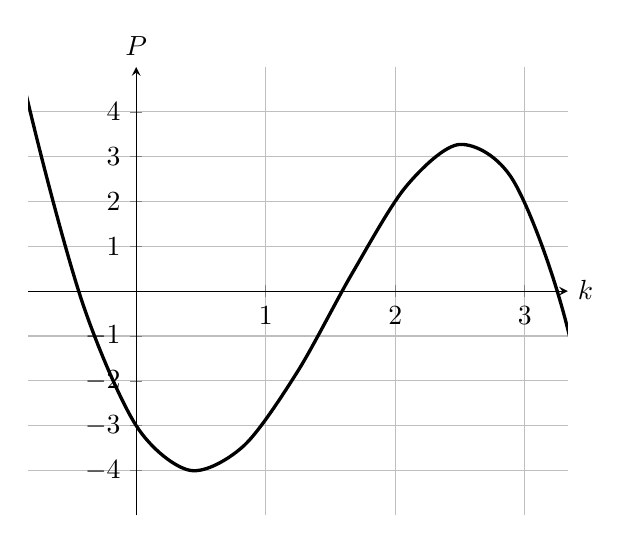
\begin{tikzpicture}
\begin{axis}[
            ymin=-5,
			ymax=5,
            axis lines =center, xlabel=$k$, ylabel=$P$,
              every axis y label/.style={at=(current axis.above origin),anchor=south},
              every axis x label/.style={at=(current axis.right of origin),anchor=west},
            domain=-5:5,
            grid = major,
            xtick={-4,...,4},
            ytick={-4,...,4},
          ]
          \addplot [very thick, smooth] {1 + (3.5 + x)*(-0.5714285714285714 + (-3.5 + x)*(0.16326530612244897 + (-0.3327149041434756 + (-0.20522334808049095 + 0.04019472590901159*(-3 + x))*(-2 + x))*x))};
        \end{axis}
\end{tikzpicture}
\]
\begin{multiple-choice}
\choice[correct]{Yes.}
\choice{No.}
\end{multiple-choice}
\begin{solution}
\begin{hint}
For each input, how many outputs are there?
\end{hint}
\end{solution}
Use the plot to compute $P(2)$
\begin{solution}
\begin{hint}
To start, find $2$ on the horizontal axis. 
\end{hint}
\begin{hint}
Now from this position, move up or down until you reach the curve. The value of $P(2)$ is the height of the curve at the point $k=2$.
\end{hint}
The value of $P(2)$ is \answer{$2$}.
\end{solution}
\end{question}


\begin{question}
In the plot below, is $R$ a function of $n$?
\[
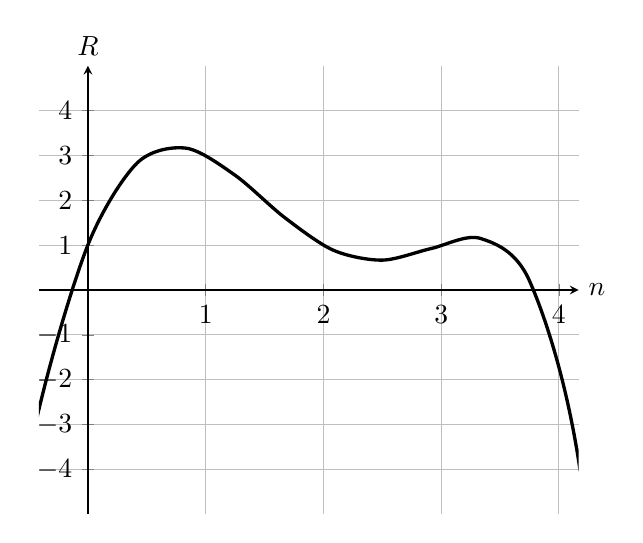
\begin{tikzpicture}
\begin{axis}[
            ymin=-5,
			ymax=5,
            axis lines =center, xlabel=$n$, ylabel=$R$,
              every axis y label/.style={at=(current axis.above origin),anchor=south},
              every axis x label/.style={at=(current axis.right of origin),anchor=west},
            domain=-5:5,
            grid = major,
            xtick={-4,...,4},
            ytick={-4,...,4},
          ]
          \addplot [very thick, smooth] {4 + (-0.42857142857142855 + (-0.05952380952380952 + (0.09163059163059163 + (-0.041447441447441453 - 0.08955488955488956*(-3 + x))*(-2 + x))*(-0.5 + x))*(-3.5 + x))*(3.5 + x)};
        \end{axis}
\end{tikzpicture}
\]
\begin{multiple-choice}
\choice[correct]{Yes.}
\choice{No.}
\end{multiple-choice}
\begin{solution}
\begin{hint}
For each input, how many outputs are there?
\end{hint}
\end{solution}
Use the plot to compute $R(3)$
\begin{solution}
\begin{hint}
To start, find $3$ on the horizontal axis. 
\end{hint}
\begin{hint}
Now from this position, move up or down until you reach the curve. The value of $R(3)$ is the height of the curve at the point $n=3$.
\end{hint}
The value of $R(3)$ is \answer{$1$}.
\end{solution}
\end{question}

\begin{question}
In the plot below, is $b$ a function of $w$?
\[
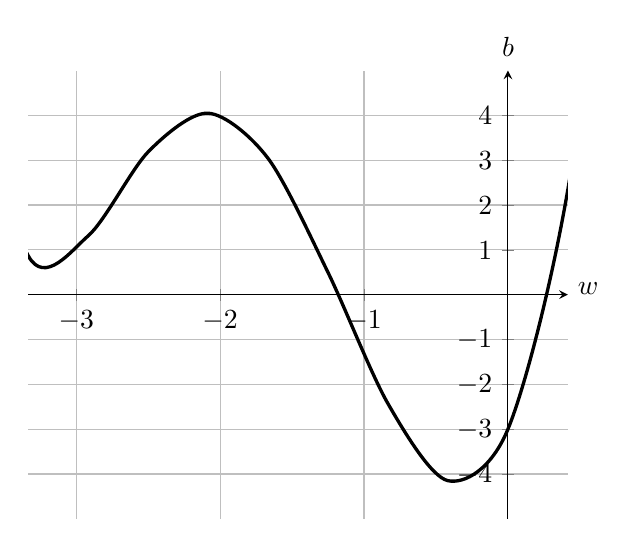
\begin{tikzpicture}
\begin{axis}[
            ymin=-5,
			ymax=5,
            axis lines =center, xlabel=$w$, ylabel=$b$,
              every axis y label/.style={at=(current axis.above origin),anchor=south},
              every axis x label/.style={at=(current axis.right of origin),anchor=west},
            domain=-5:5,
            grid = major,
            xtick={-4,...,4},
            ytick={-4,...,4},
          ]
          \addplot [very thick, smooth] {2 + (3.5 + x)*(0.2857142857142857 + (-3.5 + x)*(0.489795918367347 + x*(0.34013605442176864 + (-0.5850340136054422 - 0.25117739403453676*(-0.5 + x))*(2 + x))))};
        \end{axis}
\end{tikzpicture}
\]
\begin{multiple-choice}
\choice[correct]{Yes.}
\choice{No.}
\end{multiple-choice}
\begin{solution}
\begin{hint}
For each input, how many outputs are there?
\end{hint}
\end{solution}
Use the plot to compute $b(-2)$
\begin{solution}
\begin{hint}
To start, find $-2$ on the horizontal axis. 
\end{hint}
\begin{hint}
Now from this position, move up or down until you reach the curve. The value of $b(-2)$ is the height of the curve at the point $w=-2$.
\end{hint}
The value of $b(-2)$ is \answer{$4$}.
\end{solution}
\end{question}
\end{shuffle}






%%%%%%%%%%%%%%%%%%%%%%%%%%%%%%%%%%%%%%%%%%%%%%%%%%%%%%%%%%%%
%%%%%%%%%%%%%%%%%%%%%%%%%%%%%%%%%%%%%%%%%%%%%%%%%%%%%%%%%%%%
%% Problem
%%%%%%%%%%%%%%%%%%%%%%%%%%%%%%%%%%%%%%%%%%%%%%%%%%%%%%%%%%%%
%%%%%%%%%%%%%%%%%%%%%%%%%%%%%%%%%%%%%%%%%%%%%%%%%%%%%%%%%%%%


\begin{question} 
Suppose you are standing on a bridge that is 60 meters above
sea-level. You toss a ball up into the air with an initial velocity of
30 meters per second.  If $t$ is the time (in seconds) after we toss
the ball, then the height at time $t$ is approximately $f(t) = -5 t^2
+30t+60$. What does $f(2)$ mean in our context?
\begin{solution}
\begin{hint}
We want an answer in the context of the problem. 
\end{hint}
\answer[free-response]{The value $f(2)$ is the height of the ball after $2$ seconds.}
\end{solution}
Now suppose $t$ is such that $f(t) = 100$. What does this mean in our
context?
\begin{solution}
\begin{hint}
We want an answer in the context of the problem. 
\end{hint}
\answer[free-response]{These value of $t$ are the times when the ball is at 100 meters above sea level.}
\end{solution}
Finally, if $h$ is a small positive value what is the meaning of
$f(t+h)$? How does this compare to the meaning of $f(t)+h$?
\begin{solution}
\begin{hint}
We want an answer in the context of the problem. 
\end{hint}
\answer[free-response]{The value $f(t+h)$ gives the height of the ball
  slightly after time $t$. On the other hand, the value $f(t)+h$ gives
  a height just higher than the ball at time $t$.}
\end{solution}
\end{question}


